\section{Thống kê mô tả}

\subsection{Bảng thống kê mẫu}
\begin{figure}[H]
    \centering
    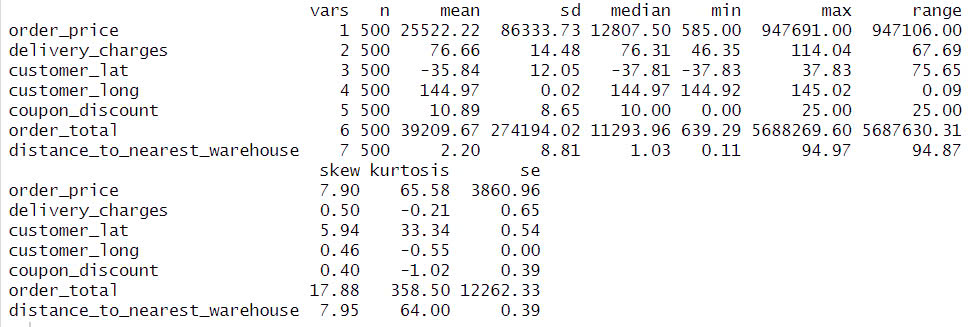
\includegraphics[width=0.8\linewidth]{graphics/bảng thống kê mẫu.jpg}
    \caption{Bảng thống kê mẫu}
    \label{34}
\end{figure}
\textbf{Nhận xét:} Từ bảng thống kê hình \ref{34} 
chúng ta có những cái nhìn tổng quan về dữ liệu như: số lượng quan sát \textbf{n}, trung bình mẫu \textbf{mean}, trung vị \textbf{median}, độ lệch chuẩn \textbf{sd}, khoảng biến thiên \textbf{range}, sai số chuẩn \textbf{se}, độ lệch \textbf{skew}, đánh giá độ nhọn \textbf{kurtosis}


\subsection{Phân tích biến liên tục bằng biểu đồ.}
\subsubsection{Đồ thị Histogram}
	Vì chúng ta làm phân tích các ảnh hướng đến chi phí đơn hàng và vì chúng ta đã sử dụng biến distance\_to\_nearest\_warehouse nên chúng ta sẽ không cần dùng tới biến customer\_lat và customer-\\\_long. Dưới đây là một số hình ảnh của các biến order\_price, delivery\_charges, coupon\_dis-count, order\_total, distance\_to\_nearest\_warehouse. Khi biểu diễn bằng đồ thị Histogram
\begin{figure}[H]
    \centering
    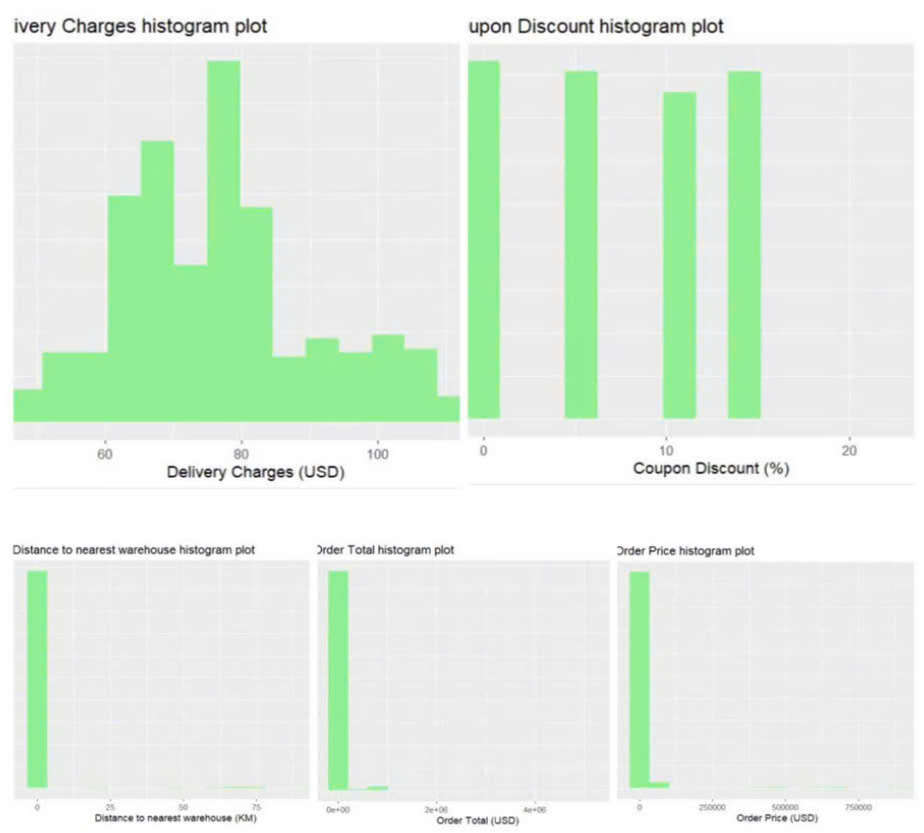
\includegraphics[width=0.7\linewidth]{graphics/bang7.jpg}
    \caption{Đồ thị Histogram của các biến liên tục}\
    \label{asb}
\end{figure}
\FloatBarrier

\textbf{Nhận xét}: Từ đồ thị hình \ref{asb} cho thấy biến order\_total, order\_price, distance\_to\_nearest\_ware-house có phân phối lệch phải, với một cột cao ở phía bên trái. Điều này cho thấy hầu hết khách hàng chỉ chi tiêu ở mức thấp hơn, trong khi một số ít có tổng giá trị đơn hàng cao, tạo ra các điểm ngoại lệ. Phân phối lệch phải thường cho thấy  rằng có một số khách hàng chi tiêu rất cao, điều này có thể ảnh hưởng đến quy mô hình hồi quy. Sau khi kiểm tra tỉ lệ khuyết nhỏ của các ngoại lai .Để xử lí tình trạng phân phối lệch phải này, chúng ta áp dụng xóa bỏ các ngoại lai  của order\_total, order\_price, distance\_to\_nearest\_warehouse.


 Đồ thị hình \ref{abs} là đồ thị các biến liên tục sau khi xóa ngoại lai.
 \begin{figure}[H]
    \centering
    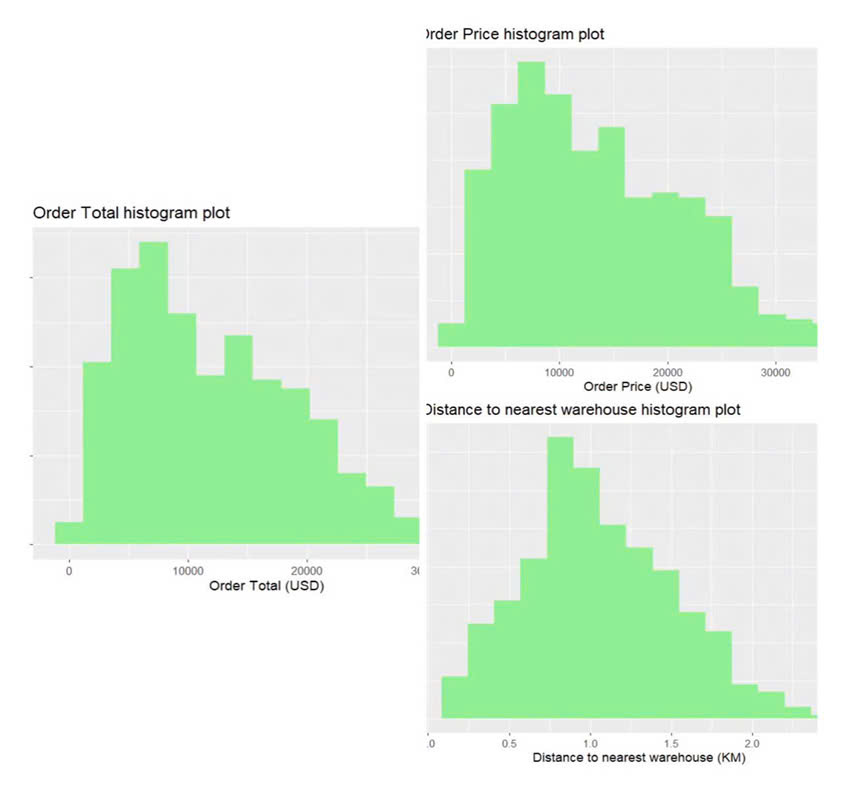
\includegraphics[width=0.7\linewidth]{graphics/bang8.jpg}
    \caption{Đồ thị Histogram của các biến liên tục đã xóa ngoại lai}
    \label{abs}
\end{figure}
\subsubsection{Đồ thị phân tán}
Chúng ta so sánh  lần lượt từng order\_price, delivery\_charges, coupon\_discount, distance\_to\_near-est\_warehouse với order\_total. Với những đồ thị có những chấm màu xanh là chưa xóa ngoại lai, còn những đồ thị có chấm màu đỏ là đã xóa ngoại lai.
\begin{figure}[!htbp]
    \centering
    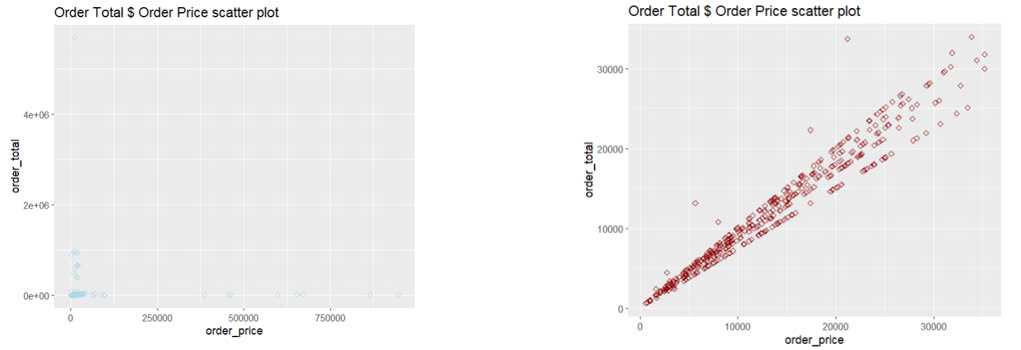
\includegraphics[width=0.85\linewidth]{graphics/bang9.jpg}
    \caption{Hình chưa xóa ngoại lai và đã xóa của order\_price}
    \label{a}
\end{figure}
\begin{figure}[!htbp]
    \centering
    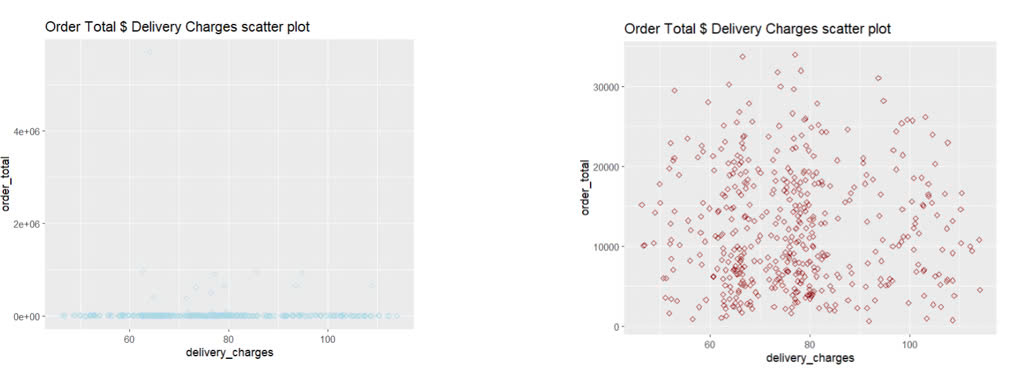
\includegraphics[width=0.8\linewidth]{graphics/bang10.jpg}
    \caption{Hình chưa xóa ngoại lai và đã xóa của delivery\_charges}
    \label{b}
\end{figure}
\begin{figure}[!htbp]
    \centering
    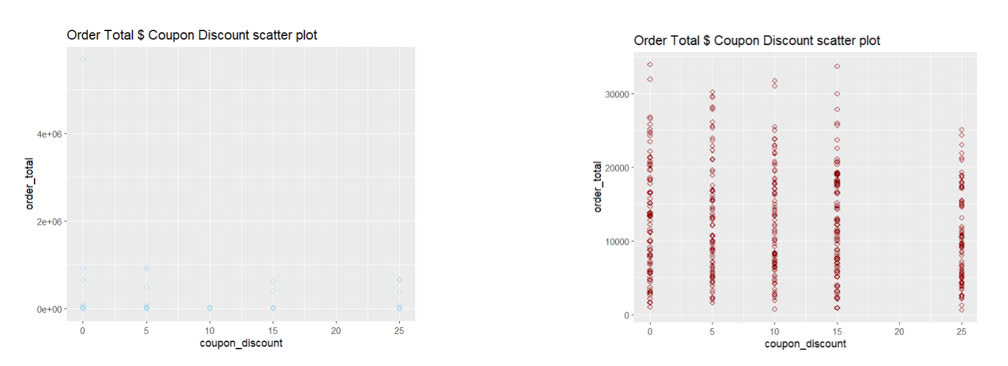
\includegraphics[width=0.8\linewidth]{graphics/bang11.jpg}
    \caption{Hình chưa xóa ngoại lai và đã xóa của coupon\_discount}
    \label{c}
\end{figure}
\begin{figure}[!htbp]
    \centering
    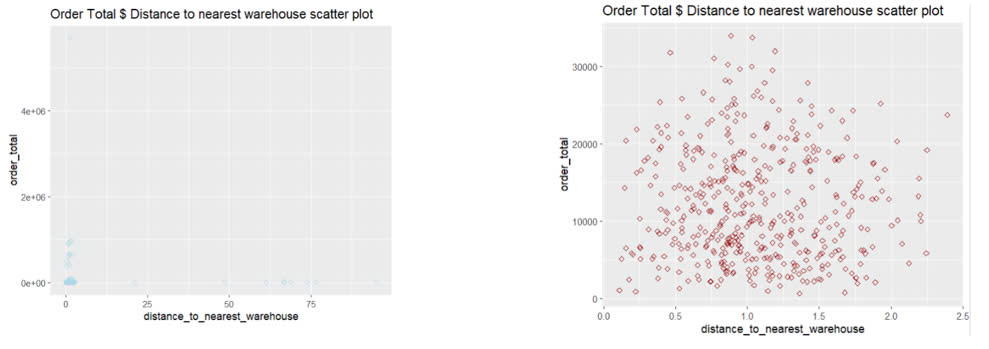
\includegraphics[width=0.8\linewidth]{graphics/bang12.jpg}
    \caption{Hình chưa xóa ngoại lai và đã xóa của distance\_to\_nearest\_warehouse}
    \label{d}
\end{figure}

\textbf{Nhận xét:} Từ 4 đồ thị hình \ref{a}, hình \ref{b}, hình \ref{c}, hình \ref{d} chúng ta rút ra được hai biến order\_price và coupon\_discount là 2 biến có ảnh hưởng tới order\_total hay còn gọi là có quan hệ tuyến tính. Hai biến delivery\_charges và distance\_to\_nearest\_warehouse không có ảnh hưởng tới order\_total hay không có quan hệ tuyến tính.

\subsection{Phân tích biến phân loại bằng biểu đồ boxplot}
Chúng ta phân tích biến order\_total theo các biến nearest\_warehouse, season, is\_expedited\_deli-very, is\_happy\_customer.
\begin{figure}[!htbp]
    \centering
    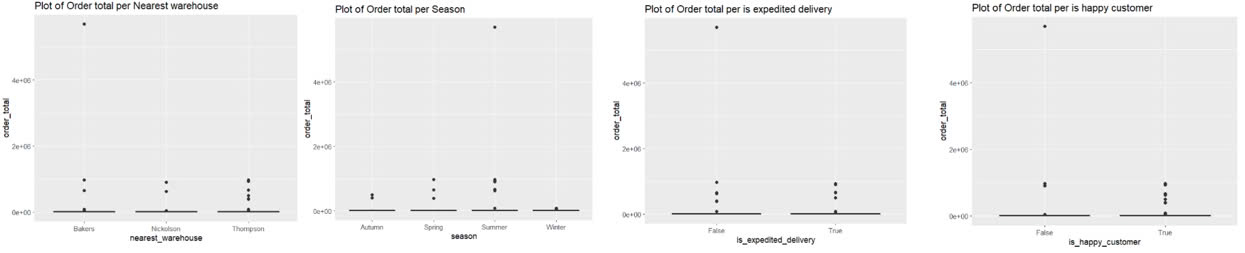
\includegraphics[width=1\linewidth]{graphics/bang13.jpg}
    \caption{Biểu đồ boxplot chưa xóa ngoại lai của các biến phân loại}
\end{figure}
\begin{figure}[!htbp]
    \centering
 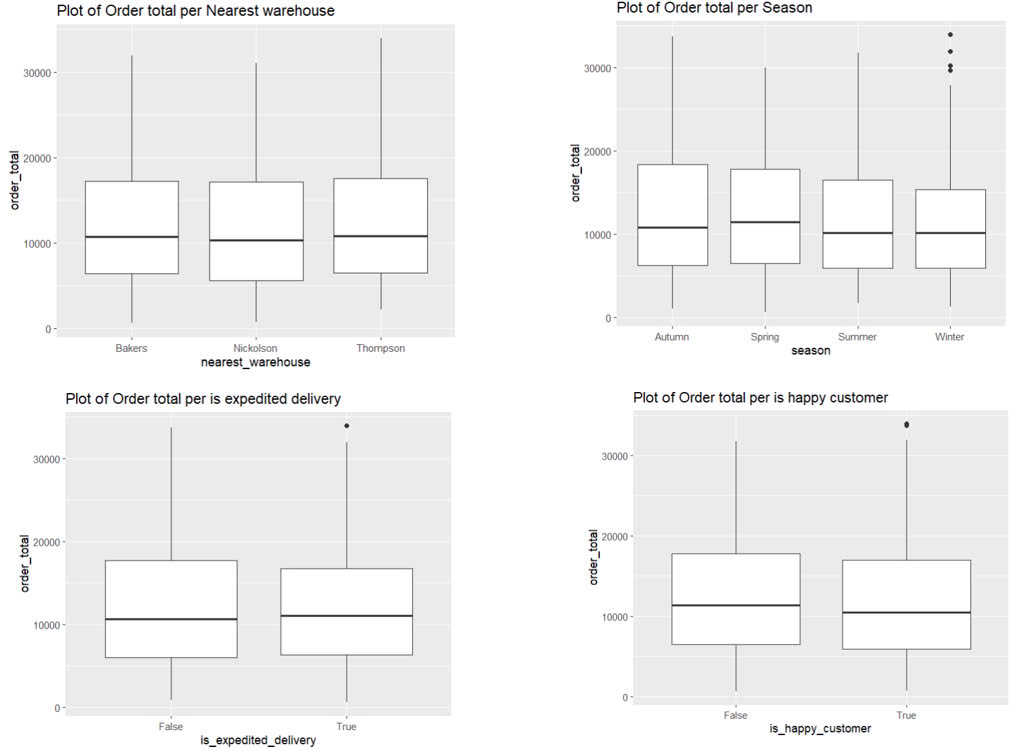
\includegraphics[width=0.9\linewidth]{graphics/bang14.jpg}
 \caption{Biểu đồ boxplot đã xóa ngoại lai của các biến phân loại}
 \label{e}
\end{figure}


\textbf{Nhận xét:} Từ đồ thị hình \ref{e}
\begin{itemize}
    \item Cả ba kho hàng (Bakers, Nickolson, Thompson) đều có phân bố tổng đơn hàng tương tự nhau, với các giá trị trung vị (median) gần như ngang bằng.
    \item Phân bố giá trị order\_total khá đồng đều qua các mùa, tuy nhiên mùa Đông có một vài đơn hàng nổi bật với giá trị rất lớn.
    \item Hình thức giao hàng nhanh dường như không có ảnh hưởng rõ rệt đến tổng giá trị đơn hàng trong phần lớn các trường hợp.
    \item Trạng thái hài lòng của khách hàng không tạo ra sự khác biệt lớn trong tổng giá trị đơn hàng, nhưng nhóm khách hàng hài lòng có xu hướng chi tiêu nhiều hơn một chút và có thể thực hiện các đơn hàng có giá trị rất lớn (outliers).
\end{itemize}


\subsection{Bảng tương quan giữa các biến}
Bảng đánh giá tương quan trong đồ thị trên được sử dụng để hiểu rõ mối quan hệ giữa các biến số trong tập dữ liệu.

\begin{figure}[!htbp]
    \centering
    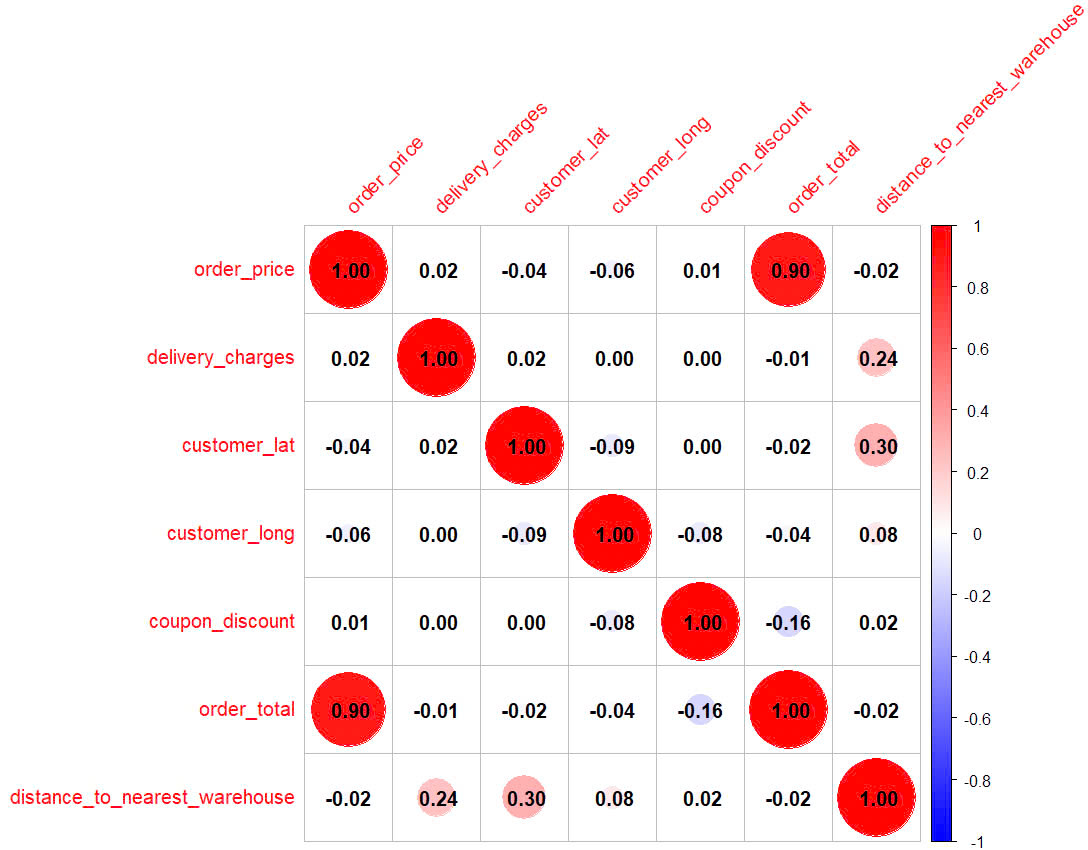
\includegraphics[width=0.8\linewidth]{graphics/tq.jpg}
    \caption{Biểu đồ tương quan của các biến}
    \label{fig:4.9}
\end{figure}
\newpage
\textbf{Nhận Xét:} Từ đồ thị hình \ref{fig:4.9}
\begin{itemize}
    \item order\_price và order\_total (tương quan: +0.90):
    Đây là mối tương quan dương mạnh. Khi giá trị của order\_price tăng, order\_total cũng tăng mạnh theo và ngược lại. Điều này dễ hiểu vì order\_price là một thành phần chính của order\_total.
    
    \item distance\_to\_nearest\_warehouse và customer\_lat (+0.30):
    Có mối tương quan dương trung bình giữa khoảng cách đến kho hàng và vĩ độ của khách hàng. Điều này có thể ngụ ý rằng vị trí kho hàng có xu hướng gần các khu vực cụ thể về mặt địa lý.
    
    \item distance\_to\_nearest\_warehouse và delivery\_charges (+0.24):
    Mối tương quan dương nhẹ cho thấy khoảng cách đến kho hàng có tác động nhỏ đến chi phí giao hàng. Khoảng cách lớn hơn thường đi kèm với phí giao hàng cao hơn.
    
    \item order\_price và delivery\_charges (+0.02):
    Hầu như không có mối liên hệ giữa giá trị đơn hàng và phí giao hàng. Điều này có thể chỉ ra rằng phí giao hàng không phụ thuộc vào giá trị đơn hàng mà dựa trên các yếu tố khác như khoảng cách hoặc chính sách giao hàng.
    
    \item coupon\_discount với hầu hết các biến khác (gần 0):
    Mức giảm giá từ phiếu coupon không có mối liên hệ đáng kể với bất kỳ biến nào trong tập dữ liệu, kể cả order\_total. Điều này có thể ngụ ý rằng chiến lược giảm giá không ảnh hưởng rõ ràng đến hành vi mua sắm của khách hàng.
\end{itemize}